\title[Applying Newton's Laws]{Applying Newton's Laws}
\subtitle{Mechanics Practice Session · \labversionlabel}
\author{}
\institute{}
\date{}
\newif\iflabforces
\labforcesfalse
\newcommand{\labfigure}[2][]{%
  \begingroup#1\centering
  \resizebox{\linewidth}{!}{\input{figures/#2.tikz}}\par
  \endgroup}
\newcommand{\modelnote}[1]{\par\smallskip{\footnotesize\textbf{Model:} #1}\par}

\begin{document}
% The title uses the same unchanged campus and logo assets as the earlier labs.
\begin{frame}[plain]
  \begin{tikzpicture}[remember picture,overlay]
    \node[anchor=north west,inner sep=0pt] at (current page.north west) {
      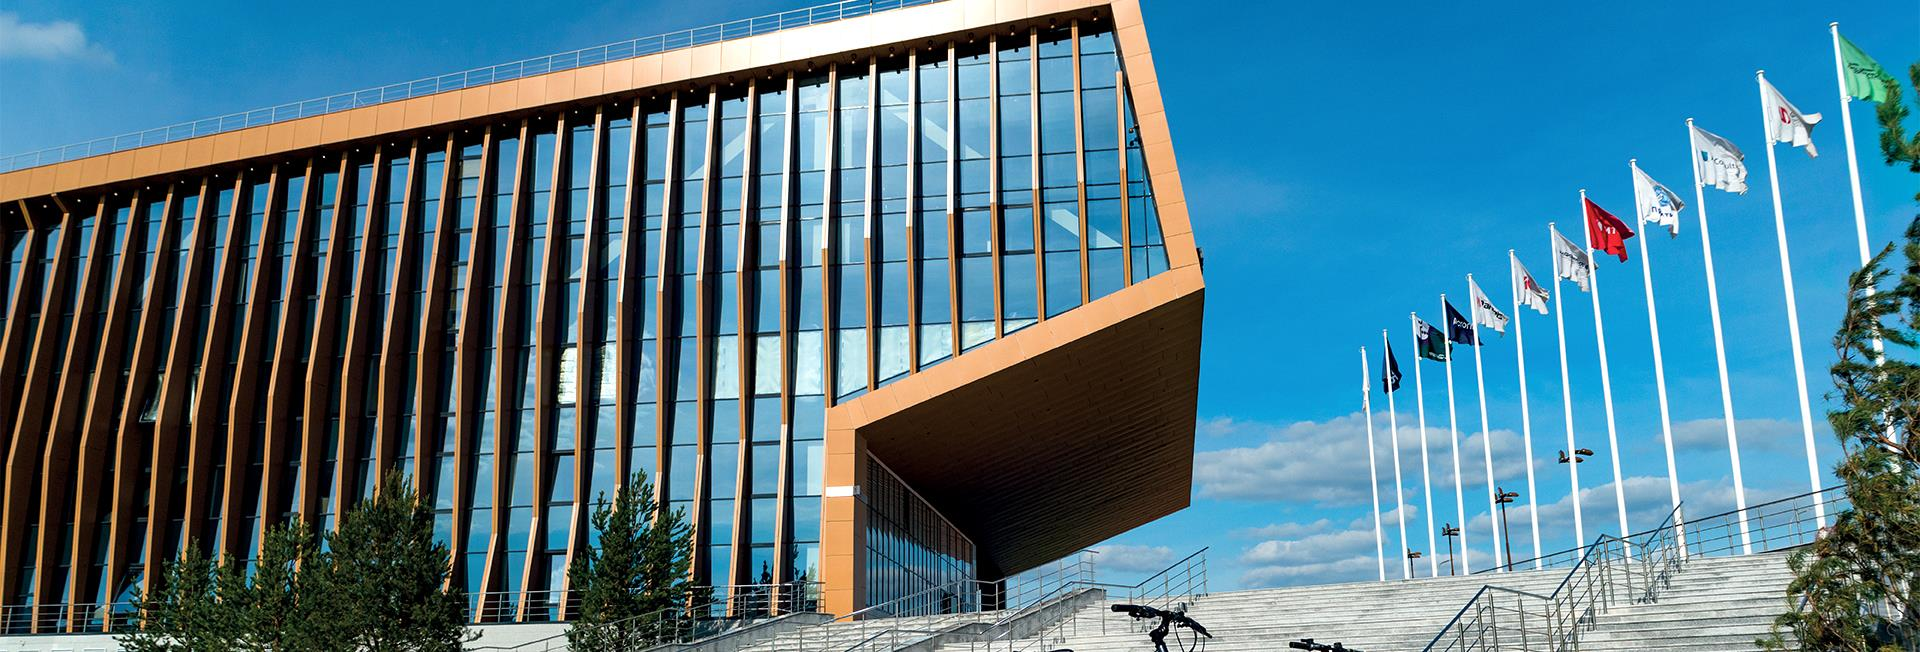
\includegraphics[width=\paperwidth,height=0.58\paperheight]
        {assets/innopolis-campus.jpg}};
    \fill[white] (current page.south west) rectangle
      ([yshift=-0.58\paperheight]current page.north east);
    \fill[PhysicsBlue] (current page.south west) rectangle
      ([xshift=0.012\paperwidth,yshift=-0.58\paperheight]current page.north west);
    \node[anchor=north west,text width=0.86\paperwidth,align=left]
      at ([xshift=0.055\paperwidth,yshift=-0.64\paperheight]current page.north west) {
      {\color{PhysicsBlue}\small\bfseries MECHANICS PRACTICE SESSION\par}
      \vspace{0.45em}
      {\color{PhysicsInk}\fontsize{17}{20}\selectfont\bfseries Applying Newton's Laws\par}
      \vspace{0.55em}
      {\color{PhysicsMuted}\small\labversionlabel\par}};
    \node[anchor=east,inner sep=0pt]
      at ([xshift=-0.055\paperwidth,yshift=0.16\paperheight]current page.south east) {
      
\includegraphics[width=0.20\paperwidth]{assets/innopolis-university-logo.png}};
  \end{tikzpicture}
\end{frame}

% T01--T04: editorial theory requested by the user on 2026-09-26.
\begin{frame}{Newton's Second Law}
  \slidetag{THEORY}\par
  For a body of constant mass in an inertial reference frame,
  \begin{block}{Net force determines acceleration}
    \[
      \mathbf F_{\mathrm{net}}=\sum\mathbf F_{\mathrm{ext}}=m\mathbf a.
    \]
  \end{block}
  \begin{itemize}
    \item Add all external forces \textbf{as vectors}.
    \item Acceleration points along the net force, not necessarily
      along the velocity.
    \item For the same net force, a larger mass gives a smaller acceleration.
  \end{itemize}
  \medskip
  \textbf{Zero net force:} \(\mathbf a=\mathbf 0\), so velocity is constant;
  the body may be at rest or moving.
\end{frame}

\begin{frame}{Applying the Second Law}
  \slidetag{THEORY}\par
  \small
  \begin{columns}[T,onlytextwidth]
    \begin{column}{.55\textwidth}
      \begin{enumerate}
        \item Choose the body and an inertial frame.
        \item Draw only the forces \emph{on that body}.
        \item Choose axes; resolve each force.
        \item Write one equation per axis.
      \end{enumerate}
      \medskip
      \textbf{Example:} a block slides right along a fixed level surface.
      The pull \(F\) is horizontal.
      \[
        \begin{aligned}
          F-\mathrm{fr}&=ma_x,\\
          N-mg&=ma_y=0.
        \end{aligned}
      \]
    \end{column}
    \begin{column}{.41\textwidth}
      \labfigure{newton-second-law}
      \smallskip
      \textbf{Here} \(N=mg\), because the vertical forces balance.
      The sign of \(F-\mathrm{fr}\) determines whether the block speeds up
      or slows down.
    \end{column}
  \end{columns}
\end{frame}

\begin{frame}{What Is Friction?}
  \slidetag{THEORY}\par
  Friction \(\vec{\mathrm{fr}}\) acts \textbf{parallel to the surface};
  the normal force \(N\) is perpendicular to it.
  \begin{block}{Choose the direction from relative motion}
    Friction opposes sliding, or the tendency to slide,
    between the two surfaces in contact.
  \end{block}
  \begin{itemize}
    \item Microscopic adhesion and deformation of surface irregularities
      contribute to friction.
    \item Static friction can accelerate a box along with an accelerating
      belt, without slipping.
    \item Find \(N\) from the force equations first; it is not always \(mg\).
  \end{itemize}
  \medskip
  For sliding, the force magnitude is \(\mathrm{fr}=\mu N\).
  The coefficient \(\mu\) is dimensionless and depends on the surfaces.
\end{frame}

\begin{frame}{Types of Friction}
  \slidetag{THEORY}\par
  \small
  \renewcommand{\arraystretch}{1.25}
  \begin{tabularx}{\textwidth}{@{}
      >{\raggedright\arraybackslash}p{.19\textwidth}
      >{\raggedright\arraybackslash}p{.30\textwidth}
      >{\raggedright\arraybackslash}X@{}}
    \toprule
    \textbf{Type} & \textbf{Contact condition} & \textbf{Force or mechanism} \\
    \midrule
    \textbf{Static}\newline (no slipping)
      & No relative sliding at the contact.
      & \(0\le \mathrm{fr}\le\mu_sN\). Adjusts as needed; equality only at the limit. \\
    \addlinespace[.25em]
    \textbf{Kinetic}\newline (sliding)
      & Surfaces slide relative to each other.
      & \(\mathrm{fr}=\mu_kN\), opposite relative sliding. \\
    \addlinespace[.25em]
    \textbf{Rolling}\newline resistance
      & A wheel or ball rolls on a surface.
      & Energy loss through deformation; not the sliding-friction law. \\
    \bottomrule
  \end{tabularx}
  \medskip
  Here \(\mathrm{fr}=|\vec{\mathrm{fr}}|\); \(s\) and \(k\) label static and kinetic
  coefficients. Typically \(\mu_k\le\mu_s\); the model is approximate.

  \medskip
  \textbf{Rolling without slipping} can involve static friction.
  This is distinct from rolling resistance.
\end{frame}

% P01: F1, S1. Approved modeling clarification M01.
\begin{frame}{Problem 1 — Two Rough Surfaces}
  \slidetag{PROBLEM 1}\par
  \small
  An object of mass \(\SI{4.0}{\kilogram}\), starting from rest,
  slides down an incline and then along a rough horizontal surface.
  \medskip
  \begin{columns}[T,onlytextwidth]
    \begin{column}{.53\textwidth}
      \begin{itemize}
        \item Incline length: \(L_1=\SI{3.0}{\metre}\).
        \item Angle: \(\theta=\ang{30}\).
        \item Kinetic friction on the incline: \(\mu_1=0.2\).
        \item Kinetic friction on the horizontal: \(\mu_2=0.3\).
      \end{itemize}
      \begin{block}{Find}
        The horizontal distance \(L_2\) before it stops.
      \end{block}
    \end{column}
    \begin{column}{.43\textwidth}
      \labfigure{two-rough-surfaces}
    \end{column}
  \end{columns}
  \modelnote{Sliding begins as stated. The transition to the horizontal
    introduces no additional loss of speed.}
\end{frame}

\begin{solutionframe}[Solution 1 — Motion Down the Incline]
  \begin{columns}[T,onlytextwidth]
    \begin{column}{.56\textwidth}
      Take \(+x\) down the incline and \(+y\) normal to it.
      There is no normal acceleration:
      \[
        N=mg\cos\theta,\qquad \mathrm{fr}=\mu_1N.
      \]
      Newton's second law along the incline gives
      \[
        ma_1=mg\sin\theta-\mu_1mg\cos\theta,
      \]
      \[
        a_1=g(\sin\theta-\mu_1\cos\theta).
      \]
      Starting from rest, \(v^2=2a_1L_1\), so
      \answer{\(\displaystyle v^2=2gL_1(\sin\theta-\mu_1\cos\theta).\)}
    \end{column}
    \begin{column}{.40\textwidth}
      \labfigure[\labforcestrue]{two-rough-surfaces}
      \medskip
      Friction opposes sliding. The blue acceleration arrow is not a force.

      \medskip
      \textbf{Check:} \(\tan\ang{30}>\mu_1\), so the downslope acceleration is positive.
    \end{column}
  \end{columns}
\end{solutionframe}

\begin{solutionframe}[Solution 1 — Stopping on the Horizontal]
  \begin{columns}[T,onlytextwidth]
    \begin{column}{.58\textwidth}
      With \(+x\) to the right, \(N=mg\) and
      \(a_x=-\mu_2g\). Define the positive deceleration \(b=\mu_2g\).
      \[
        0=v^2-2bL_2
        \quad\Longrightarrow\quad
        L_2=\frac{v^2}{2\mu_2g}.
      \]
      Substituting the symbolic result from the incline,
      \[
        L_2=\frac{L_1}{\mu_2}
          (\sin\theta-\mu_1\cos\theta).
      \]
      Only now insert the data:
      \[
        L_2=\frac{\SI{3.0}{\metre}}{0.3}
          (\sin\ang{30}-0.2\cos\ang{30}).
      \]
    \end{column}
    \begin{column}{.38\textwidth}
      \labfigure{horizontal-stopping}
      \answer{\(\displaystyle L_2\approx\SI{3.27}{\metre}.\)}
      \medskip
      \textbf{Check:} mass and \(g\) cancel; the result has units of length.
      Greater horizontal friction shortens the stopping distance.
    \end{column}
  \end{columns}
\end{solutionframe}

% P02: F4, S2. M02--M03 fix the model and reference frame explicitly.
\begin{frame}{Problem 2 — A Wedge and a Bar}
  \slidetag{PROBLEM 2}\par
  \small
  \begin{columns}[T,onlytextwidth]
    \begin{column}{.53\textwidth}
      A bar of mass \(m\) slides down the vertical face of a wedge of mass
      \(M\). The kinetic friction coefficient is \(\mu\).

      \medskip
      The rope follows the two pulleys as shown.
      \begin{block}{Find}
        The bar's acceleration relative to the ground.
      \end{block}

      \modelnote{The ground is smooth. The taut rope is massless and
      inextensible; the pulleys are ideal and attached to the wedge.
      The right end is fixed to the ground. The bar remains in contact.}
    \end{column}
    \begin{column}{.43\textwidth}
      \labfigure{moving-wedge-pulleys}
    \end{column}
  \end{columns}
\end{frame}

\begin{solutionframe}[Solution 2 — The Rope Constraint]
  \begin{columns}[T,onlytextwidth]
    \begin{column}{.42\textwidth}
      \labfigure[\labforcestrue]{moving-wedge-pulleys}
    \end{column}
    \begin{column}{.54\textwidth}
      Let \(X\) be the wedge position and \(y\) the bar height,
      measured in the ground frame. Use \(+x\) right and \(+y\) up.
      \[
        h=h_0-y,\qquad s=s_0-X,
      \]
      \[
        h+s+\text{constant}=\ell
        \quad\Rightarrow\quad \ddot y=-\ddot X.
      \]
      The other rope sections move with the wedge and keep their lengths.

      \medskip
      Set \(A=\ddot X>0\). The bar stays against the face:
      \[
        a_x=A,\qquad a_y=-A.
      \]
      Thus \(N=mA\); friction on the bar acts upward,
      with magnitude \(\mathrm{fr}=\mu N\).
    \end{column}
  \end{columns}
\end{solutionframe}

\begin{solutionframe}[Solution 2 — Acceleration in the Ground Frame]
  \begin{columns}[T,onlytextwidth]
    \begin{column}{.58\textwidth}
      For the whole system, the only external horizontal force is the
      fixed-end rope tension:
      \[
        T=(M+m)A,\qquad N=mA.
      \]
      For the bar, with \(+y\) upward,
      \[
        \begin{gathered}
          T+\mu N-mg=-mA,\\[.4em]
          [M+(2+\mu)m]A=mg,\qquad
          A=\frac{mg}{M+(2+\mu)m}.
        \end{gathered}
      \]
    \end{column}
    \begin{column}{.38\textwidth}
      \labfigure{wedge-bar-freebody}
      \medskip
      Relative to the wedge,
      \(\mathbf a_{\rm rel}=-A\hat{\mathbf j}\), with magnitude \(A\).
    \end{column}
  \end{columns}
  \answer{\(\displaystyle
    \mathbf a=A\hat{\mathbf i}-A\hat{\mathbf j},\qquad
    |\mathbf a|=\sqrt2 A=\frac{\sqrt2\,mg}{M+(2+\mu)m}.
  \)}
\end{solutionframe}

% P03: F6, S3. M04: kinetic friction during steady sliding.
\begin{frame}{Problem 3 — The Best Pulling Angle}
  \slidetag{PROBLEM 3}\par
  \small
  \begin{columns}[T,onlytextwidth]
    \begin{column}{.54\textwidth}
      A packing crate of unknown mass is pulled across the floor at
      constant velocity by a cable.

      \medskip
      The angle \(\theta_0\) corresponds to the minimum pulling force.

      \medskip
      \begin{block}{Find}
        The friction coefficient between the crate and the floor.
      \end{block}

      \modelnote{The crate is already sliding, with kinetic friction,
      and remains in contact with the floor.}
    \end{column}
    \begin{column}{.42\textwidth}
      \labfigure{crate-pulling}
      \medskip
      \(\theta\) is a variable pulling angle; \(\theta_0\) is its optimum.
    \end{column}
  \end{columns}
\end{frame}

\begin{solutionframe}[Solution 3 — Force as a Function of Angle]
  \begin{columns}[T,onlytextwidth]
    \begin{column}{.56\textwidth}
      Constant velocity means zero acceleration, so
      \[
        F\cos\theta=\mathrm{fr}=\mu N,\qquad
        N+F\sin\theta=mg.
      \]
      The upward component of the pull reduces the normal reaction:
      \[
        F\cos\theta=\mu(mg-F\sin\theta).
      \]
      Therefore
      \answer{\(\displaystyle F(\theta)=
        \frac{\mu mg}{\cos\theta+\mu\sin\theta}.\)}
    \end{column}
    \begin{column}{.40\textwidth}
      \labfigure[\labforcestrue]{crate-pulling}
      \medskip
      For \(0\le\theta<\pi/2\), the denominator is positive.
      With \(\mu>0\), minimizing \(F\) means maximizing this denominator.
    \end{column}
  \end{columns}
\end{solutionframe}

\begin{solutionframe}[Solution 3 — Finding the Optimum]
  \begin{columns}[T,onlytextwidth]
    \begin{column}{.53\textwidth}
      Write \(S(\theta)=\cos\theta+\mu\sin\theta\).
      \[
        S'(\theta_0)=-\sin\theta_0+\mu\cos\theta_0=0.
      \]
      Thus
      \answer{\(\mu=\tan\theta_0.\)}
      Since \(S''=-S<0\), this is a maximum of the denominator,
      hence a minimum of the required force.

      \medskip
      At the optimum, \(N=mg/(1+\mu^2)>0\), so contact is maintained.
    \end{column}
    \begin{column}{.43\textwidth}
      \labfigure{pulling-force-optimum}
      \medskip
      The mass cancels; the graph specifies no numerical \(\mu\).

      \medskip
      \textbf{Degenerate case:} if \(\mu=0\), no force is needed
      at any angle. There is no unique optimal angle.
    \end{column}
  \end{columns}
\end{solutionframe}

% P04: F8, S4. M05 is the idealization used by the source solution.
\begin{frame}{Problem 4 — Maximum Height Uphill}
  \slidetag{PROBLEM 4}\par
  \small
  \begin{columns}[T,onlytextwidth]
    \begin{column}{.54\textwidth}
      A man rides a skateboard. His initial speed at the foot of a hill
      is \(v_0\), directed up the slope.

      \medskip
      The hill makes an angle \(\alpha\) with the horizontal,
      and the friction coefficient is \(\mu\).

      \medskip
      \begin{block}{Find}
        What maximum vertical height \(H\) will he reach?
      \end{block}

      \modelnote{Treat rider and board as one translating body, with
      resistance \(\mathrm{fr}=\mu N\). Neglect wheel rotational energy.
      Assume \(0<\alpha<\pi/2\).}
    \end{column}
    \begin{column}{.42\textwidth}
      \labfigure{uphill-motion}
    \end{column}
  \end{columns}
\end{frame}

\begin{solutionframe}[Solution 4 — From Stopping Distance to Height]
  \begin{columns}[T,onlytextwidth]
    \begin{column}{.60\textwidth}
      With \(+x\) uphill, \(N=mg\cos\alpha\) and
      \[
        ma_x=-mg\sin\alpha-\mathrm{fr},\qquad \mathrm{fr}=\mu N.
      \]
      Set \(b=-a_x=g(\sin\alpha+\mu\cos\alpha)>0\).
      \[
        t_{\rm stop}=\frac{v_0}{b},\qquad
        S=v_0t_{\rm stop}-\frac12bt_{\rm stop}^2
          =\frac{v_0^2}{2b}.
      \]
      The requested height is \(H=S\sin\alpha\):
    \end{column}
    \begin{column}{.36\textwidth}
      \labfigure[\labforcestrue]{uphill-motion}
      \medskip
      \textbf{Checks:} \(\mu=0\) gives \(H=v_0^2/(2g)\).
      The shortcut \(S=bt^2/2\) holds here only after using \(v_0=bt_{\rm stop}\).
    \end{column}
  \end{columns}
  \answer{\(\displaystyle H=\frac{v_0^2\sin\alpha}
    {2g(\sin\alpha+\mu\cos\alpha)}
    =\frac{v_0^2}{2g(1+\mu\cot\alpha)}.\)}
\end{solutionframe}

% P05: F10, S5. M06 clarifies the first stop and static retention.
\begin{frame}{Problem 5 — Position-Dependent Friction}
  \slidetag{PROBLEM 5}\par
  \small
  \begin{columns}[T,onlytextwidth]
    \begin{column}{.54\textwidth}
      A bar starts from rest and slides down a plane inclined at
      angle \(\alpha\). Its kinetic friction coefficient varies as
      \[
        \mu(x)=fx,\qquad f>0,
      \]
      where \(x\) is distance along the slope from the start.

      \begin{block}{Find}
        (a) The total distance travelled.\\
        (b) The maximum speed.
      \end{block}

    \end{column}
    \begin{column}{.42\textwidth}
      \labfigure{variable-friction-incline}
      \medskip
      Here \(f\) is the constant spatial gradient of \(\mu(x)\),
      with units \(\si{\per\metre}\).
    \end{column}
  \end{columns}
  \modelnote{The slope is long enough and \(0<\alpha<\pi/2\).
    At the first stop, the static friction coefficient is at least
    the local kinetic coefficient, so the bar can remain at rest.}
\end{frame}

\begin{solutionframe}[Solution 5 — From Time to Position]
  \begin{columns}[T,onlytextwidth]
    \begin{column}{.60\textwidth}
      Take \(+x\) downslope. With \(N=mg\cos\alpha\) and
      \(\mathrm{fr}=\mu(x)N\), Newton's law gives
      \[
        a=g(\sin\alpha-fx\cos\alpha).
      \]
      \textbf{Why is \(a=v\frac{dv}{dx}\)?}
      Speed depends on position, and position depends on time:
      \(v=v(x(t))\). Apply the chain rule:
      \[
        a=\frac{dv}{dt}
        =\frac{dv}{dx}\frac{dx}{dt}
        =v\frac{dv}{dx},
        \qquad \frac{dx}{dt}=v.
      \]
      \(\frac{dv}{dx}\) measures speed change per metre.
      Multiplying by \(\frac{dx}{dt}=v\) gives speed change per second.
    \end{column}
    \begin{column}{.36\textwidth}
      \labfigure[\labforcestrue]{variable-friction-incline}
      \medskip
      Use this relation while the bar slides downslope, with \(v>0\).
      The values at the start and the stop follow by continuity.
    \end{column}
  \end{columns}
\end{solutionframe}

\begin{solutionframe}[Solution 5 — Why the Speed Is Squared]
  \par
  Rearrange \(a=v\frac{dv}{dx}\) as \(v\,dv=a(x)\,dx\).
  Starting at \(x=0\) with \(v=0\), integrate:
  \[
    \int_0^{v(x)}v\,dv
      =g\int_0^x(\sin\alpha-f\xi\cos\alpha)\,d\xi.
  \]
  \textbf{The square comes from integrating \(v\,dv\):}
  \(\frac{d}{dv}\left(\frac{v^2}{2}\right)=v\).
  Evaluating both integrals gives
  \[
    \frac{v^2(x)-0^2}{2}
      =g\left[\xi\sin\alpha-\frac{f\xi^2\cos\alpha}{2}\right]_0^x
      =g\left(x\sin\alpha-\frac{fx^2\cos\alpha}{2}\right).
  \]
  Here \(\xi\) is a dummy position variable. Multiply both sides by two:
  \answer{\(\displaystyle v^2(x)=g(2x\sin\alpha-fx^2\cos\alpha).\)}
\end{solutionframe}

\begin{solutionframe}[Solution 5 — Finding the Total Distance]
  \par
  At the first stop after release, \(x=D\) and \(v(D)=0\).
  Substitute these values into the speed equation:
  \[
    0=g(2D\sin\alpha-fD^2\cos\alpha)
      =gD(2\sin\alpha-fD\cos\alpha).
  \]
  One root is \(D=0\): the \emph{initial} position at rest.
  For the later stop, \(D>0\), so divide by \(gD\):
  \[
    2\sin\alpha-fD\cos\alpha=0
    \quad\Rightarrow\quad fD\cos\alpha=2\sin\alpha.
  \]
  \answer{\(\displaystyle D=\frac{2\sin\alpha}{f\cos\alpha}
      =\frac{2\tan\alpha}{f}.\)}
  \textbf{Why is this the total distance?}
  The bar moves only downslope before stopping, so the distance equals \(D\).
  At the stop, \(\mu(D)=fD=2\tan\alpha\).
  The given \(\mu_s(D)\ge\mu(D)>\tan\alpha\) lets static friction hold it there.
\end{solutionframe}

\begin{solutionframe}[Solution 5 — Where Does the Speed Peak?]
  \begin{columns}[T,onlytextwidth]
    \begin{column}{.59\textwidth}
      \textbf{1. Friction grows along the slope.}
      \(N=mg\cos\alpha\) is constant, so \(\mathrm{fr}=fxN\) grows
      with \(x\), while \(mg\sin\alpha\) stays constant:
      \[
        a(x)=g(\sin\alpha-fx\cos\alpha).
      \]
      \textbf{2. Locate the peak: set \(a(x_*)=0\).}
      \[
        \sin\alpha=fx_*\cos\alpha
        \quad\Rightarrow\quad
        x_*=\frac{\sin\alpha}{f\cos\alpha}=\frac D2.
      \]
      On the downslope branch, \(v>0\):
      \begin{itemize}
        \item \(x<x_*\): \(a>0\), so speed increases.
        \item \(x>x_*\): \(a<0\), so speed decreases.
      \end{itemize}
    \end{column}
    \begin{column}{.37\textwidth}
      \labfigure{variable-friction-speed}
      \medskip
      \textbf{At \(x_*\): \(a=0\), but \(v>0\).}
      Speed is greatest here, not zero.
    \end{column}
  \end{columns}
\end{solutionframe}

\begin{solutionframe}[Solution 5 — Calculating the Maximum Speed]
  \par
  \textbf{3. Substitute into} \(v^2(x)=g(2x\sin\alpha-fx^2\cos\alpha)\).
  \[
    \begin{aligned}
      v_{\max}^2=v^2(x_*)
        &=g\left[2\frac{\sin\alpha}{f\cos\alpha}\sin\alpha
          -f\left(\frac{\sin\alpha}{f\cos\alpha}\right)^2\cos\alpha\right]\\[.4em]
        &=g\left[\frac{2\sin^2\alpha}{f\cos\alpha}
          -\frac{\sin^2\alpha}{f\cos\alpha}\right]
          =\frac{g\sin^2\alpha}{f\cos\alpha}.
    \end{aligned}
  \]
  Take the positive square root, using \(0<\alpha<\pi/2\):
  \answer{\(\displaystyle v_{\max}=\sin\alpha
      \sqrt{\frac{g}{f\cos\alpha}}.\)}
\end{solutionframe}

% P06: F13, S6. M07 makes the source's two-regime model explicit.
\begin{frame}{Problem 6 — A Plank and a Bar}
  \slidetag{PROBLEM 6}\par
  \small
  \begin{columns}[T,onlytextwidth]
    \begin{column}{.54\textwidth}
      A plank of mass \(m_1\) lies on a smooth horizontal plane.
      A bar of mass \(m_2\) rests on it.

      \medskip
      A horizontal force \(F=pt\), with constant \(p>0\), acts on the
      \emph{bar}. The friction coefficient between the bodies is \(\mu\).

      \medskip
      \begin{block}{Find}
        The accelerations \(a_1(t)\) and \(a_2(t)\).
      \end{block}

      \modelnote{There is initially no relative sliding. Use the same
      \(\mu\) for limiting static and kinetic friction. Take \(t\ge0\);
      the results apply while the bar remains on the plank.}
    \end{column}
    \begin{column}{.42\textwidth}
      \labfigure{plank-bar-forces}
      \medskip
      \(p\) has units \(\si{\newton\per\second}\).
    \end{column}
  \end{columns}
\end{frame}

\begin{solutionframe}[Solution 6 — Which Forces Act?]
  \begin{columns}[T,onlytextwidth]
    \begin{column}{.60\textwidth}
      In the ground frame, take \(+x\) to the right.

      \medskip
      \textbf{The force \(F=pt\) pulls only the bar.}
      It tends to slide right relative to the plank, so:
      \begin{itemize}
        \item on the bar \(m_2\), friction acts left;
        \item on the plank \(m_1\), friction acts right and makes it accelerate.
      \end{itemize}
      These friction forces have equal magnitudes \(\mathrm{fr}\)
      and opposite directions (Newton's third law).

      \medskip
      The bar has no vertical acceleration:
      \[
        N-m_2g=0\quad\Rightarrow\quad N=m_2g.
      \]
      Use this contact force in \(\mu N\).
    \end{column}
    \begin{column}{.36\textwidth}
      \labfigure[\labforcestrue]{plank-bar-forces}
      \medskip
      Smooth ground: no horizontal friction.
      Its vertical support force is \(N_g\).
    \end{column}
  \end{columns}
\end{solutionframe}

\begin{solutionframe}[Solution 6 — Before Sliding: One Acceleration]
  \par
  \textbf{No relative sliding means the bodies move together:}
  their velocities stay equal, so \(a_1=a_2=a\).
  Static friction prevents sliding \emph{between the bodies};
  both bodies can still move relative to the ground.

  \medskip
  Write Newton's second law for each body, taking right as positive:
  \[
    \begin{aligned}
      \text{Plank:}\qquad m_1a&=\mathrm{fr},\\[.3em]
      \text{Bar:}\qquad m_2a&=pt-\mathrm{fr}.
    \end{aligned}
  \]
  Add the equations. The two internal friction forces cancel:
  \[
    m_1a+m_2a=\mathrm{fr}+pt-\mathrm{fr}
    \quad\Rightarrow\quad (m_1+m_2)a=pt.
  \]
  \answer{\(\displaystyle a_1(t)=a_2(t)=\frac{pt}{m_1+m_2}
    \quad\text{while there is no relative sliding}.\)}
  The applied force grows with time, so this common acceleration also grows.
\end{solutionframe}

\begin{solutionframe}[Solution 6 — When Does Sliding Begin?]
  \par
  The plank needs friction \(\mathrm{fr}=m_1a\) to share the bar's acceleration.
  Substitute \(a=pt/(m_1+m_2)\) and compare with the static-friction limit:
  \[
    \underbrace{\mathrm{fr}(t)=\frac{m_1pt}{m_1+m_2}}_{\text{required; grows with time}}
    \ \le\ \underbrace{\mu N=\mu m_2g}_{\text{available limit; constant}}.
  \]
  \textbf{At \(t=t_*\), the required friction reaches the limit.}
  Set the two sides equal:
  \[
    \frac{m_1pt_*}{m_1+m_2}=\mu m_2g
    \quad\Rightarrow\quad m_1pt_*=\mu m_2g(m_1+m_2).
  \]
  Divide by \(pm_1\):
  \answer{\(\displaystyle t_*=\frac{\mu m_2g(m_1+m_2)}{pm_1}.\)}
  For \(t>t_*\), the required friction exceeds the limit, so the bar slides forward on the plank.
\end{solutionframe}

\begin{solutionframe}[Solution 6 — During Sliding: Two Accelerations]
  \par
  For \(t>t_*\), use kinetic friction:
  \(\mathrm{fr}=\mu N=\mu m_2g\), constant in this model.
  Keep \(+x\) to the right, but now allow \(a_1\ne a_2\).

  \medskip
  \begin{columns}[T,onlytextwidth]
    \begin{column}{.47\textwidth}
      \textbf{Plank \(m_1\): friction pulls right.}
      It is the only horizontal force:
      \[
        m_1a_1=\mathrm{fr}=\mu m_2g.
      \]
      Divide by the plank's mass \(m_1\):
      \answer{\(\displaystyle a_1=\frac{\mu m_2g}{m_1}.\)}
      Constant friction gives constant acceleration.
    \end{column}
    \begin{column}{.49\textwidth}
      \textbf{Bar \(m_2\): pull right, friction left.}
      The resultant force is their difference:
      \[
        m_2a_2=pt-\mathrm{fr}=pt-\mu m_2g.
      \]
      Divide by the bar's mass \(m_2\):
      \answer{\(\displaystyle a_2(t)=\frac{pt}{m_2}-\mu g.\)}
      The pull keeps growing; friction stays fixed. The acceleration grows.
    \end{column}
  \end{columns}
  \medskip
  Velocities agree at \(t_*\). Since \(a_2-a_1=p(t-t_*)/m_2>0\), the bar pulls ahead.
\end{solutionframe}

\begin{solutionframe}[Solution 6 — Choosing the Right Formula]
  \par
  Each body has one acceleration function with two time intervals:
  use the common-motion formula up to \(t_*\), then the sliding formula.

  \medskip
  \begin{columns}[T,onlytextwidth]
    \begin{column}{.48\textwidth}
      \textbf{Plank \(m_1\)}
      \answer{\(\displaystyle
        a_1(t)=
        \begin{cases}
          \dfrac{pt}{m_1+m_2},&0\le t\le t_*,\\[.7em]
          \dfrac{\mu m_2g}{m_1},&t>t_*.
        \end{cases}
      \)}
    \end{column}
    \begin{column}{.48\textwidth}
      \textbf{Bar \(m_2\)}
      \answer{\(\displaystyle
        a_2(t)=
        \begin{cases}
          \dfrac{pt}{m_1+m_2},&0\le t\le t_*,\\[.7em]
          \dfrac{pt}{m_2}-\mu g,&t>t_*.
        \end{cases}
      \)}
    \end{column}
  \end{columns}
  \medskip
  The switching time is
  \(\displaystyle t_*=\frac{\mu m_2g(m_1+m_2)}{pm_1}.\)
  \medskip

  \textbf{Keep \(t\) and \(t_*\) distinct:}
  \(t\) is the current time; \(t_*\) is a fixed threshold set by the data.
  The formulas apply while the bar remains on the plank.
\end{solutionframe}

\begin{solutionframe}[Solution 6 — Reading the Acceleration Graph]
  \begin{columns}[T,onlytextwidth]
    \begin{column}{.40\textwidth}
      \labfigure{plank-bar-accelerations}
      \[
        a_1(t_*)=a_2(t_*)=\frac{\mu m_2g}{m_1}\equiv a_*.
      \]
    \end{column}
    \begin{column}{.56\textwidth}
      \textbf{Before \(t_*\):} one rising line for both bodies,
      since \(a_1=a_2=pt/(m_1+m_2)\).

      \medskip
      \textbf{After \(t_*\), plank:} a horizontal line.
      Its friction force and acceleration are constant.
      Constant acceleration means a constant rate of change of velocity.

      \medskip
      \textbf{After \(t_*\), bar:} a steeper rising line.
      Its slope is \(p/m_2\), greater than the earlier
      \(p/(m_1+m_2)\).

      \medskip
      \textbf{The curves meet at \(a_*\).} There is no jump because the model
      uses the same \(\mu\) for limiting static and kinetic friction.
      At \(t=0\), both accelerations are zero.
    \end{column}
  \end{columns}
\end{solutionframe}
\end{document}
